\documentclass[a4paper,10pt,oneside]{article}
%
% This is a basic set of packages.  Feel free to use as many packages
% as you want, only the generated PDF will be submitted in the end.
%
\usepackage[utf8]{inputenc}
\usepackage{amsmath,amssymb}
\usepackage{subcaption}
\usepackage{xcolor,graphicx}
%
% Page layout (DO NOT CHANGE)
%
\usepackage[margin=32mm]{geometry}
\setlength{\parindent}{0em}
\setlength{\parskip}{1.3ex plus 0.5ex minus 0.2ex}
%
% Size of section titles (DO NOT CHANGE)
%
\usepackage{titlesec}
\titleformat*{\section}{\large\bfseries}
%
% MASCOT header (DO NOT CHANGE)
%
\usepackage{fancyhdr}
\pagestyle{fancy}
\fancyhead[L]{MASCOT-NUM 2024}
\fancyhead[C]{}
\fancyhead[R]{April 3--5, Hy\`eres, France}
%
% Well, as you can guess, this is where you must enter the
% title of your communication:
%
\title{%
  Data assimilation method for particle-based simulations} % : EnKF adaptations and optimal transport perpectives}
%
% Here, as you can guess too, is the place for the list of authors.
% Since this is a template for the PhD student's day, it is expected
% that the first author should be a PhD student...
%
\author{%
  M. Duvillard${}^{\dagger,1,2}$, %
  L. Giraldi${}^{\S,1}$, %
  O. Le Maître${}^{\S,2}$}%
%
\date{\medskip%
  %
  % In this block, you only have to indicate the expected PhD duration:
  % *REMOVE THE RED MARK*
  %
  \small %
  ${}^\dagger$\ PhD student (presenting author). \quad ${}^{\S}$\ PhD supervisors\\[5pt]
  PhD expected duration: {Oct. 2021 -- Sep. 2024}\\[15pt]
  %
  % Of course, edit this:
  %
  ${}^1$  CEA, DES, IRESNE, DEC, SESC, F-13108 Saint-Paul-lez-Durance, France\\
  \texttt{\{marius.duvillard,loic.giraldi\}@cea.fr}\\[4pt]
  ${}^2$ CNRS, Inria, Centre de Mathématiques Appliquées, Ecole Polytechnique, IPP, Route de Saclay, 91128, Palaiseau Cedex, France\\
  \texttt{olivier.le-maitre@polytechnique.edu}}
% rajouter platon.
%
\newcommand{\loic}[1]{{\color{red}#1}}
\newcommand{\marius}[1]{{\color{green}#1}}

\newcommand{\cL}{\mathcal{L}}
\newcommand{\xs}{X^\star}

\begin{document}

\maketitle

\thispagestyle{fancy}

\section*{Abstract}

Particle-based methods are simulation approaches that rely on Lagrangian representations capable of handling complex geometries with large deformations and changes in the shape of a continuum (such as fragmentation and free-surface flow).
These methods discretize the continuous fields and operator using an ensemble of particles (computational elements) that move according to a velocity field. The Vortex Method (VM) is one such method dedicated to solving incompressible fluid dynamics~\cite{book_vortex}. A typical particle approximation $\hat{\omega}$ of a field $\omega(z)$ writes as
\[
  \omega(z) \approx \hat{\omega} (z) = \sum_{p=1}^m \Gamma_p \phi(z-z_p),
\]
where $m$ is the number of particles, $z_p$ is the position of the $p$-th particle, $\Gamma_p$ is its weight, and $\phi$ is the kernel of the approximation.

This work aims to propose new data assimilation methods adapted for particle-based simulations. Data assimilation concerns the update of the model state using sequential observations. Generally, the assimilation problem is formulated either with a variational approach (minimization of a cost function), a Bayesian approach (estimation of the model state's posterior distribution), or a hybridization of the two previous approaches~\cite{evensen_data_2022}.

A state-of-the-art Bayesian filter is the ensemble approximation of the Kalman filter known as Ensemble Kalman Filters (EnKF). EnKF methods propagate an ensemble of states to estimate the covariance of the Gaussian forecast distribution (before assimilation) and compute the associated Kalman gain. EnKF methods apply to high-dimensional non-linear systems without suffering from the curse of dimensionality (thanks to low-rank approximations of the covariance matrices).

Standard EnKF methods use an identical discretization (computational grid) for all members, allowing simple linear combinations of members to define the corrections. This restriction has led our work to introduce two adaptations of this filter. They are based either on the remeshing of each particle discretization on a common one (Remesh-EnKF) or by a projection of the analyzed solution on each particle discretization (Part-EnKF). The two filters are evaluated on a two-dimensional incompressible fluid flow with the estimation of a model parameter as illustrated in Figure~\ref{fig:vortex}. We show that the Remesh-EnKF outperforms the result due to difficulties for the Part-EnKF in representing the analyzed solution.

This issue arises from the fact that the support of the particle discretization of the members does not correspond to the analyzed solution. This mismatch is linked to a common mistake in data assimilation when an error in position occurs. A misalignment of the forecast and the ground truth leads to an over-penalization of the model and observation errors, known as the double penalty effect. Advances have been made to correct the position and the intensity of the forecast to address this issue. It is either done by introducing a displacement field to align the forecast ensemble~\cite{ravela_data_2007} or by using Optimal Transport (OT)~\cite{feyeu2016}.

The talk will be based on the presentation, and the comparison of the two filters applied to the assimilation of two-dimensional incompressible fluid flows. I will introduce correction position techniques to overcome the weakness of the filter associated with a non-adapted particle discretization support.
\begin{figure}[h]
  \centering
  \begin{subfigure}{0.35\textwidth}
    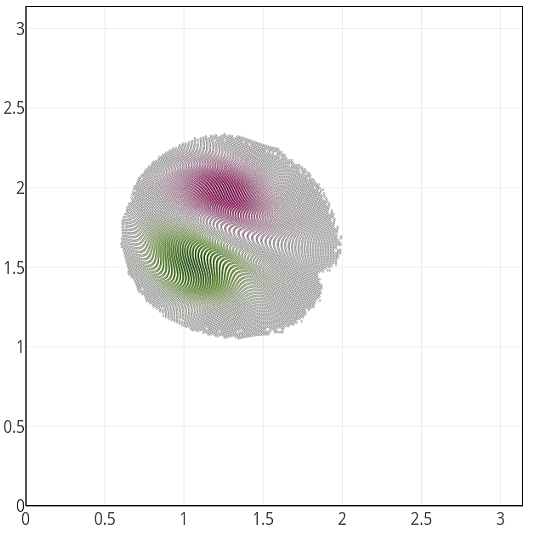
\includegraphics[width=\textwidth]{field}
  \end{subfigure}
  \hspace{1cm}
  \begin{subfigure}{0.35\textwidth}
    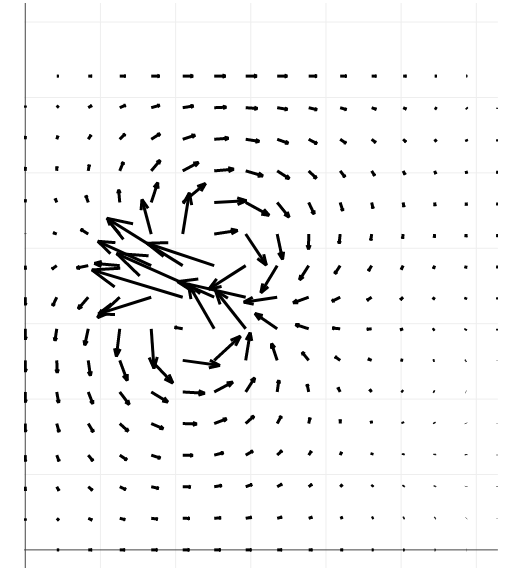
\includegraphics[width=1.02\textwidth]{velocity_2.00}
  \end{subfigure}
  \caption{\small Left: Vorticity field of the reference solution at $t = 4s$. Right: Associate observation of the velocity field.}
  \label{fig:vortex}
\end{figure}

\section*{Short biography (PhD student)}

I'm a PhD student in the CEA center of Cadarache and the Platon team at the Inria Saclay Center (CMAP). I'm currently working on the development of assimilation methods that would be adapted to a grinding mill facilities involved in the fuel manufacturing process.

\bibliographystyle{plain}
\bibliography{mascotnum2024-duvillard.bib}

\end{document}
